%% BioMed_Central_Tex_Template_v1.06
%%                                      %
%  bmc_article.tex            ver: 1.06 %
%                                       %

%%IMPORTANT: do not delete the first line of this template
%%It must be present to enable the BMC Submission system to
%%recognise this template!!

%%%%%%%%%%%%%%%%%%%%%%%%%%%%%%%%%%%%%%%%%
%%                                     %%
%%  LaTeX template for BioMed Central  %%
%%     journal article submissions     %%
%%                                     %%
%%         <14 August 2007>            %%
%%                                     %%
%%                                     %%
%% Uses:                               %%
%% cite.sty, url.sty, bmc_article.cls  %%
%% ifthen.sty. multicol.sty		   %%
%%				      	   %%
%%                                     %%
%%%%%%%%%%%%%%%%%%%%%%%%%%%%%%%%%%%%%%%%%


%%%%%%%%%%%%%%%%%%%%%%%%%%%%%%%%%%%%%%%%%%%%%%%%%%%%%%%%%%%%%%%%%%%%%
%%                                                                 %%	
%% For instructions on how to fill out this Tex template           %%
%% document please refer to Readme.pdf and the instructions for    %%
%% authors page on the biomed central website                      %%
%% http://www.biomedcentral.com/info/authors/                      %%
%%                                                                 %%
%% Please do not use \input{...} to include other tex files.       %%
%% Submit your LaTeX manuscript as one .tex document.              %%
%%                                                                 %%
%% All additional figures and files should be attached             %%
%% separately and not embedded in the \TeX\ document itself.       %%
%%                                                                 %%
%% BioMed Central currently use the MikTex distribution of         %%
%% TeX for Windows) of TeX and LaTeX.  This is available from      %%
%% http://www.miktex.org                                           %%
%%                                                                 %%
%%%%%%%%%%%%%%%%%%%%%%%%%%%%%%%%%%%%%%%%%%%%%%%%%%%%%%%%%%%%%%%%%%%%%


\NeedsTeXFormat{LaTeX2e}[1995/12/01]
\documentclass[10pt]{bmc_article}



% Load packages
\usepackage{cite} % Make references as [1-4], not [1,2,3,4]
\usepackage{url}  % Formatting web addresses
\usepackage{ifthen}  % Conditional
\usepackage{multicol}   %Columns
\usepackage[utf8]{inputenc} %unicode support
\usepackage{graphicx}
\usepackage{color}
\usepackage{soul}
%\usepackage[applemac]{inputenc} %applemac support if unicode package fails
%\usepackage[latin1]{inputenc} %UNIX support if unicode package fails
\urlstyle{rm}


%%%%%%%%%%%%%%%%%%%%%%%%%%%%%%%%%%%%%%%%%%%%%%%%%	
%%                                             %%
%%  If you wish to display your graphics for   %%
%%  your own use using includegraphic or       %%
%%  includegraphics, then comment out the      %%
%%  following two lines of code.               %%
%%  NB: These line *must* be included when     %%
%%  submitting to BMC.                         %%
%%  All figure files must be submitted as      %%
%%  separate graphics through the BMC          %%
%%  submission process, not included in the    %%
%%  submitted article.                         %%
%%                                             %%
%%%%%%%%%%%%%%%%%%%%%%%%%%%%%%%%%%%%%%%%%%%%%%%%%


%\def\includegraphic{}
%\def\includegraphics{}



\setlength{\topmargin}{0.0cm}
\setlength{\textheight}{21.5cm}
\setlength{\oddsidemargin}{0cm}
\setlength{\textwidth}{16.5cm}
\setlength{\columnsep}{0.6cm}

\newboolean{publ}

%%%%%%%%%%%%%%%%%%%%%%%%%%%%%%%%%%%%%%%%%%%%%%%%%%
%%                                              %%
%% You may change the following style settings  %%
%% Should you wish to format your article       %%
%% in a publication style for printing out and  %%
%% sharing with colleagues, but ensure that     %%
%% before submitting to BMC that the style is   %%
%% returned to the Review style setting.        %%
%%                                              %%
%%%%%%%%%%%%%%%%%%%%%%%%%%%%%%%%%%%%%%%%%%%%%%%%%%


%Review style settings
%\newenvironment{bmcformat}{\begin{raggedright}\baselineskip20pt\sloppy\setboolean{publ}{false}}{\end{raggedright}\baselineskip20pt\sloppy}

%Publication style settings
%\newenvironment{bmcformat}{\fussy\setboolean{publ}{true}}{\fussy}

%New style setting
\newenvironment{bmcformat}{\baselineskip20pt\sloppy\setboolean{publ}{false}}{\baselineskip20pt\sloppy}



% Begin ...
\begin{document}
\begin{bmcformat}


%%%%%%%%%%%%%%%%%%%%%%%%%%%%%%%%%%%%%%%%%%%%%%
%%                                          %%
%% Enter the title of your article here     %%
%%                                          %%
%%%%%%%%%%%%%%%%%%%%%%%%%%%%%%%%%%%%%%%%%%%%%%

\title{BiNoM, a Cytoscape plugin for accessing and analyzing pathways using
standard systems biology formats}

%%%%%%%%%%%%%%%%%%%%%%%%%%%%%%%%%%%%%%%%%%%%%%
%%                                          %%
%% Enter the authors here                   %%
%%                                          %%
%% Ensure \and is entered between all but   %%
%% the last two authors. This will be       %%
%% replaced by a comma in the final article %%
%%                                          %%
%% Ensure there are no trailing spaces at   %%
%% the ends of the lines                    %%     	
%%                                          %%
%%%%%%%%%%%%%%%%%%%%%%%%%%%%%%%%%%%%%%%%%%%%%%


% \author{Jane E Doe\correspondingauthor$^1$%
%          \email{Jane E Doe\correspondingauthor - jane.e.doe@cambridge.co.uk}
%        and
%          John RS Smith$^2$%
%          \email{John RS Smith - john.RS.Smith@cambridge.co.uk}%
%       }
%

\author{Eric Bonnet$^{1,2,3}$ \and Laurence Calzone$^{1,2,3}$ \and Daniel
Rovera$^{1,2,3}$ \and Gautier Stoll$^{1,2,3}$ Emmanuel Barillot$^{1,2,3}$ and Andrei Zinovyev$^{1,2,3}$\correspondingauthor
\email{andrei.zinovyev@curie.fr} }






%%%%%%%%%%%%%%%%%%%%%%%%%%%%%%%%%%%%%%%%%%%%%%
%%                                          %%
%% Enter the authors' addresses here        %%
%%                                          %%
%%%%%%%%%%%%%%%%%%%%%%%%%%%%%%%%%%%%%%%%%%%%%%

\address{%
    \iid(1)Institut Curie, 26 rue d'Ulm, Paris, F-75248 France\\
    \iid(2)INSERM, U900, Paris, F-75248 France\\
    \iid(3)Mines ParisTech, Fontainebleau, F-77300 France
}
\maketitle

%%%%%%%%%%%%%%%%%%%%%%%%%%%%%%%%%%%%%%%%%%%%%%
%%                                          %%
%% The Abstract begins here                 %%
%%                                          %%
%% Please refer to the Instructions for     %%
%% authors on http://www.biomedcentral.com  %%
%% and include the section headings         %%
%% accordingly for your article type.       %%
%%                                          %%
%%%%%%%%%%%%%%%%%%%%%%%%%%%%%%%%%%%%%%%%%%%%%%


\begin{abstract}

Public repositories of biological pathways and networks have greatly expanded in
recent years. Such databases contain many pathways that facilitate the analysis of high-throughput
experimental work and the formulation of new biological hypotheses to be
 tested, a fundamental principle of the Systems Biology approach.
However, large scale molecular maps are not always easy to mine and interpret. We
have developed BiNoM (Biological Network Manager), a Cytoscape plugin which provides
 functions for the import-export of standard Systems Biology
file formats, and a set of algorithms to analyze and reduce the complexity
of large biological networks. Here, we provide an in-depth overview of the BiNoM
functions, we detail novel aspects such as the support of the BioPAX level 3
format and an algorithm for the quantification of pathways for influence
networks. We also illustrate some of the BiNoM functions on a detailed biological case
study of a network representing the G1/S transition of the cell cycle.

\end{abstract}



\ifthenelse{\boolean{publ}}{\begin{multicols}{2}}{}




%%%%%%%%%%%%%%%%%%%%%%%%%%%%%%%%%%%%%%%%%%%%%%
%%                                          %%
%% The Main Body begins here                %%
%%                                          %%
%% Please refer to the instructions for     %%
%% authors on:                              %%
%% http://www.biomedcentral.com/info/authors%%
%% and include the section headings         %%
%% accordingly for your article type.       %%
%%                                          %%
%% See the Results and Discussion section   %%
%% for details on how to create sub-sections%%
%%                                          %%
%% use \cite{...} to cite references        %%
%%  \cite{koon} and                         %%
%%  \cite{oreg,khar,zvai,xjon,schn,pond}    %%
%%  \nocite{smith,marg,hunn,advi,koha,mouse}%%
%%                                          %%
%%%%%%%%%%%%%%%%%%%%%%%%%%%%%%%%%%%%%%%%%%%%%%




%%%%%%%%%%%%%%%%
%% Background %%
%%
\section*{Background}

Biological pathways and networks comprise sets of interactions, or functional
relationships, occurring at the molecular level in living cells
\cite{adriaens2008public, cary2005pathway}. 
A large body of knowledge on cellular biochemistry is organized in publicly available
repositories such as the KEGG database \cite{ogata1999kegg}, Reactome
\cite{joshi2005reactome}, MINT \cite{zanzoni2002mint}, or the Cancer Cell Map
(\url{http://cancer.cellmap.org/cellmap/}). All these pathway and biological
network databases facilitate a large spectrum of analyses, improving our
understanding of cellular systems. For example, it is now a very common
practice to cross the output of high-throughput experiments, such as mRNA or
protein expression levels, with curated biological pathways in
order to efficiently visualize changes, analyze their impact on a network and
formulate new hypotheses about
biological processes \cite{saraiya2005visualizing,
gehlenborg2010visualization}. The development of those pathway repositories has
also fueled the creation of standard representations and formats, to facilitate
the exchange and representation of data, such as the Biological Pathway
Exchange standard (BioPAX) \cite{demir2010biopax}, the Systems Biology Markup
Language (SBML) \cite{hucka2003systems} or the Systems Biology Graphical
Notation (SBGN) \cite{le2009systems}. The Pathway resource list website counts
more than 300 web-accessible biological pathway and network databases
\cite{bader2006pathguide}, many of which are using the SBML and BioPAX standard
formats. Ultimately, those integrated resources will facilitate computational
models building, their exchange, re-usability and their experimental validation, a cycle that is the
cornerstone of the Systems Biology approach \cite{karlebach2008modelling,
kitano2002systems, ideker2001new}.

As a consequence, there is a need for the precise and accurate construction of
pathways and large scale molecular maps covering fundamental biological
processes. Such maps are often constructed by manual curation of the literature or
automated curation from pathway databases \cite{bauer2009pathway}. More and more, they
are focused on the regulation of biological processes involved in diseases such
as cancer, Alzheimer's disease or Crohn's disease, to name a few \cite{oda2005comprehensive, oda2006comprehensive,
calzone2008comprehensive, caron2010comprehensive}. However, the scale of such
maps, even when they are focusing on a particular process, is quite large, with
hundreds of chemical species and interactions. The analysis and interpretation of such
large scale maps is therefore not a straightforward task. Several computational
tools have been developed to facilitate the visualization, curation and analysis
of pathways \cite{adriaens2008public}. For example, CellDesigner is a software package
for the graphical editing of biological pathway diagrams
\cite{funahashi2003celldesigner}, using a proprietary extension
of SBML to store all the information contained in the graphs. There is obviously
a need for user-friendly software tools that would allow the user to easily
import data from various standard format sources, to perform structural analyses on these pathways
and to manipulate networks, and to be able to export a network to a suitable
format for further analysis (e.g. mathematical modeling). We have created
BiNoM \cite{zinovyev2008binom}, a software plugin for the popular Cytoscape
network vizualization and analysis tool \cite{cline2007integration}. BiNoM
facilitates the usage and analysis of biological networks in standard Systems
Biology formats (SBML, SBGN, BioPAX). More specifically, BiNoM implements
several functions based on graph operations for the structural analysis of
biological networks. Those functions can be used to reduce the complexity and
extract meaningful subnetworks from large scale molecular maps. Furthermore,
BiNoM has several built-in functions for accessing standard Systems Biology file
formats. Here, we provide a detailed view on the functions implemented in BiNoM
that permit specific extraction of information from large scale molecular maps
and improve their readability and usability. We also highlight novel functions
that were implemented recently, such as the support of the latest BioPAX
specification (BioPAX level 3) and an algorithmic approach for the
quantification of pathways on influence networks (PIQuant). We illustrate the
use of the principal BiNoM functions with a detailed analysis of a molecular
netwok of the G1/S transition of the cell cycle, a central mechanism
for tumor development and progression.

\section*{Implementation}
The BiNoM software is implemented in the Java programming language, as a plugin
for the network visualization and analysis software package Cytoscape
\cite{cline2007integration}. Although the primary use of BiNoM is through the
Cytoscape software, the underlying logic of all BiNoM functions is completely
decoupled from the Cytoscape objects, allowing developers to also use BiNoM as
an independent java library \cite{zinovyev2008binom}. The installation of BiNoM
can be done through the Cytoscape plugin manager (menu ``Plugins $>$ Manage
Plugins``, section ''Analysis''), or alternatively the user can
also download the plugin together with a manual and the source code from the
BiNoM website
\url{http://binom.curie.fr/}. 


BiNoM is designed to handle different Systems Biology file formats and to
provide useful functions for the analysis of biological networks. The core
functions of BiNoM can be grouped in five different topics: Input/Output,
Analysis, BioPAX utils \& query, Module manager and Utilities.

\subsection*{BiNoM Input/Output}

BiNoM functions facilitate the import and export of standard Systems Biology
file formats, but BiNoM plugin is not designed to be a universal converter.
The goal is more
to provide robust functions for a finite number of useful conversion and
analysis scenarios, such as the examples showed below (non-exhaustive list):

\begin{itemize}

\item Interconversion of CellDesigner files to BioPAX, and from a BioPAX
reaction network to SBML level 2.

\item Import of a BioPAX file as a reaction network and/or a pathway structure
and/or a protein interactions network, followed by the creation of a subnetwork
saved as a new BioPAX file.

\item Import of a BioPAX file, selection of a subnetwork of interest saved as a SBML file for
the creation of a computational model using an appropriate software package.

\item Import a large CellDesigner map and export only a subnetwork as a new CellDesigner file.

\end{itemize}

BiNoM allows the user to import and export SBML level 2 files, as well as
CellDesigner 3.x and 4.x file formats \cite{zinovyev2008binom}. The BioPAX
community has recently made a major update of the BioPAX standard, producing a
new specification known as BioPAX Level 3 (\url{http://www.biopax.org/}). This
format supports metabolic pathways, signaling pathways (including states of molecules
and generic molecules), gene regulatory networks, molecular interactions and
genetic interactions. Due to major changes in the
specification, the BioPAX level 3 is incompatible with the level 2 file format.

BioPAX is using the web ontology language specification (OWL,
\url{http://www.w3.org/2004/OWL/}) to store data in XML-formatted files. In
BiNoM, we use the Jastor and the Jena java libraries
(\url{http://jastor.sourceforge.net/}, \url{http://jena.sourceforge.net/}) to
automatically create java classes from the BioPAX specifications, allowing a
convenient access to the different data types encoded in the BioPAX files. The
guiding principle in BiNoM for the
access to Systems Biology files is to provide control over the content without
completely converting the file to the Cytoscape format. The content is therefore
mapped to a labeled directed graph, representing the complete set of objects and
their relationships. This graph, called the index, is highly connected and is
not visualized explicitly. Instead, the user interacts with selected subgraphs
extracted from the index. For example, BioPAX files are imported as three
separate graphs, respectively the Reaction Network (RN), representing the
biochemical reaction network, the Pathway Structure (PS), showing the
hierarchical organisation of pathways, and the Interaction Map graph
(IM). Several examples of simple BioPAX level 3 files imported through BiNoM
are shown in Figure~\ref{6biopax3_examples}. Figure~\ref{apoptosishierarchical}
shows the hierarchical structure of the human Apoptosis pathway, extracted
from Reactome database, and constructed by BiNoM.


\begin{figure}[h]
 \caption{\label{6biopax3_examples}  \textbf{Visualization of the six BioPAX example files, provided in BioPAX 3.0 documentation.} 
The BioPAX 3.0 documentation available at http://biopax.org contains six simple examples of BioPAX 3.0 files that describe
different aspects of biological networks interactions (genetic interaction, short metabolic pathway, gene regulatory network, biochemical reactioni, phosphorylation, protein interaction). Here we show how BiNoM visualizes these examples
after their import. The BiNoM type of representation iis indicated below the reaction type, in backets (Reaction Network, Pathway Structureand Interaction Map). The graphical node and edge semantics 
is described in more details in the BiNoM manual.}
 \center{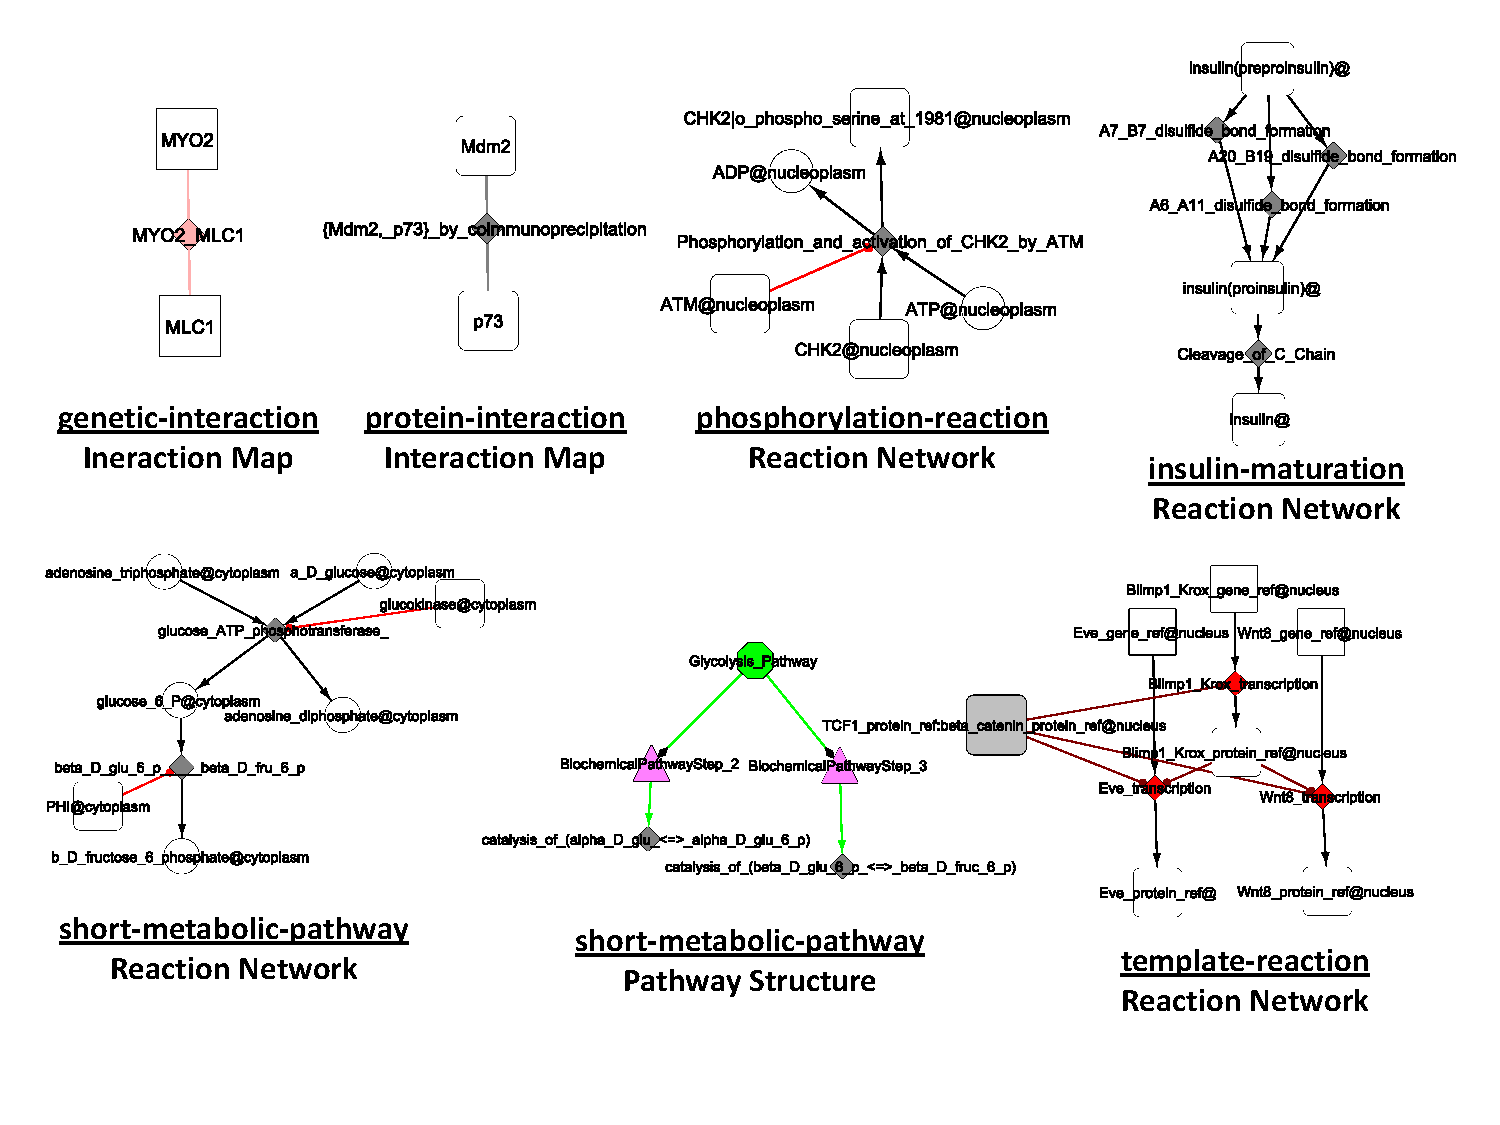
\includegraphics[width=0.9\textwidth]{figures/6biopax3_examples.pdf}}
\end{figure}

\begin{figure}[h]
 \caption{\label{apoptosishierarchical}  \textbf{Apoptosis pathway 
structure.} Representation of BioPAX data extracted from the Reactome database
\cite{joshi2005reactome}, corresponding to the Apoptosis pathway and imported through
BiNoM, using Pathway Structure BioPAX representation. The green nodes represent pathways, the pink
triangular nodes denote steps, while grey nodes indicate reactions.}
 \center{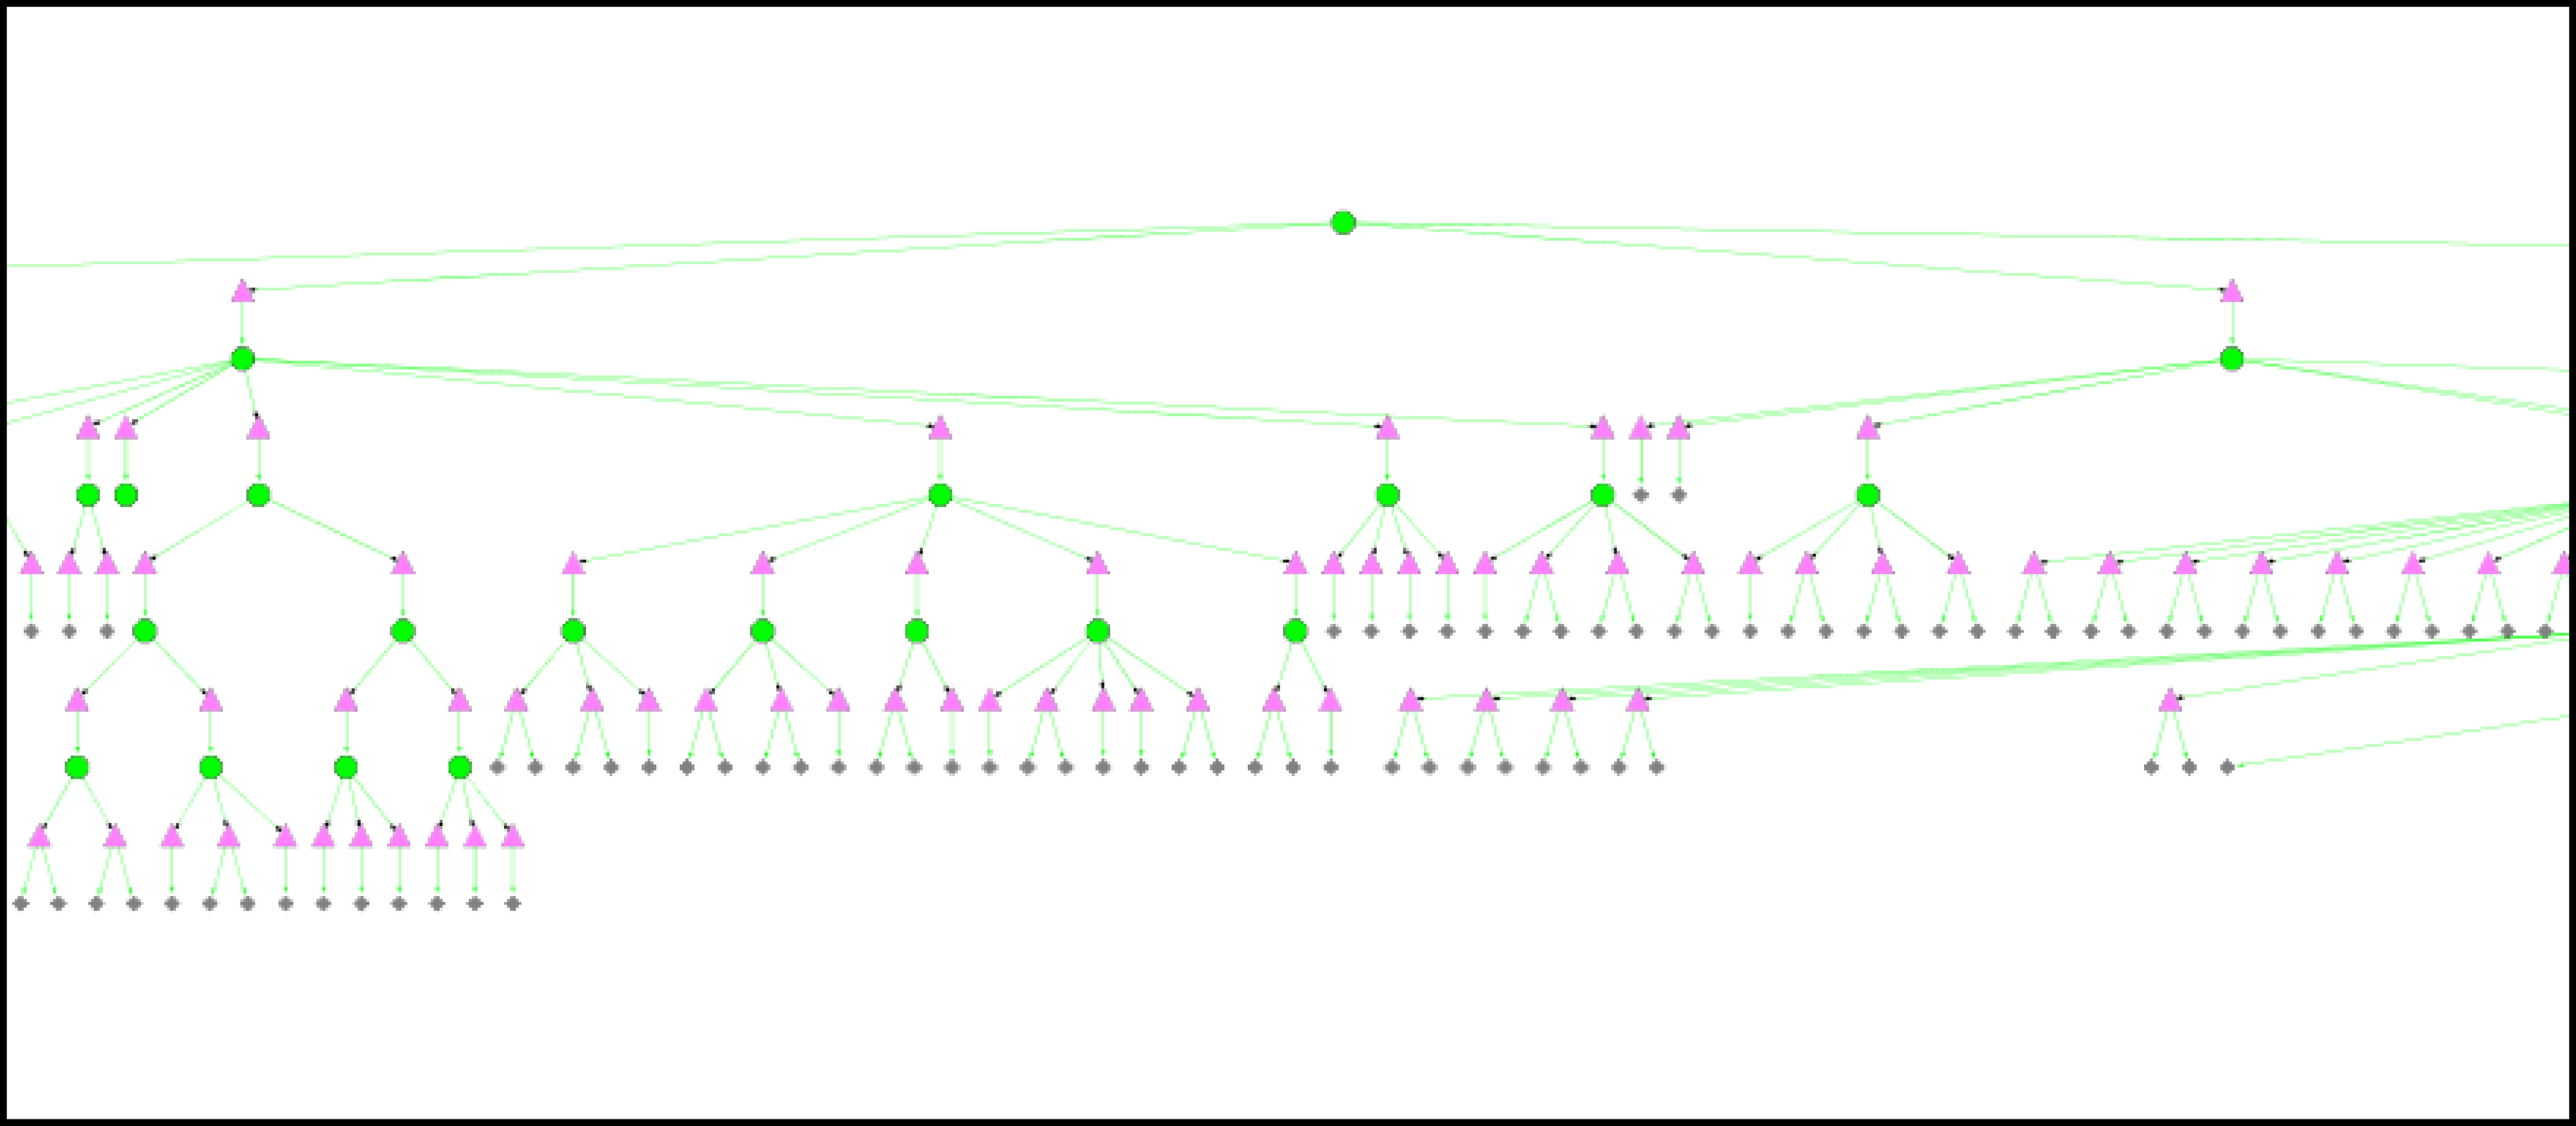
\includegraphics[width=0.9\textwidth]{figures/apoptosis_hierarchical.png}}
\end{figure}


When importing a file, BiNoM is calling a \emph{naming service} function in
order to create meaningful names for the various entities. More precisely,
entity names are combined with other features such as modifications, compartment
and complex components. The different features are indicated by special
characters, such as ``@'' for the compartments, ``$|$'' for modifications and
``:'' to delimitate the different members of a complex. For example, the
name Cdc25$|$Pho@cytoplasm represents the protein Cdc25 in a phosphorylated
state, located in the cytoplasm, while the name
Cdc13:Cdc2$|$Thr167\_pho@cytoplasm indicates a protein complex located in the
cytosplasm, composed of the protein Cdc13 and the protein Cdc2 phosphorylated at
position 167 on a threonine residue.


\subsection*{BiNoM Analysis}
The central goal of the BiNoM plugin is to provide efficient methods
and algorithms to reduce the inherent complexity of biological networks into
manageable and meaningful subnetworks. This goal is achieved by a set of
functions included as a built-in structural graph analysis library. Some of the functions take into
account the semantics contained in the graph element names.
The structural analysis functions implemented in BiNoM include the analysis of
connected and strongly connected components, pruning the network, decomposition
by involvement of a protein (material components) or by cyclic decomposition, path analysis and network clustering.
We also introduce in this version of BiNoM a novel function to quantify the
influence of a source node on a target node taking into account experimental data, called PIQuant.

\subsubsection*{Decomposition by involvement of a protein or by cyclic decomposition}

BiNoM allows many methods to dissect a complex biological network into parts.
A trivial approach to separate a network into subparts is to dissociate the unconnected subparts
of the network. A more sophisticated one consists in decomposing the network into
strongly connected components, using the algorithm of Tarjan
\cite{tarjan1972depth}. It is also possible to prune the network into three different parts:
the one with all the elements associated with the \emph{input} part of the network (from which all paths lead to the central core), the
second with all the elements associated with the \emph{output} part (from which there are no paths leading back to the central core) and the last
part with all the elements linked to the central core, cyclic part, composed from strongly connected components, possibly connected together. 
This type of approach corresponds to finding the bow-tie graph structure \cite{broder2000graph}.

The decomposition in material components is using the node name semantics to
isolate subnetworks in which each protein is involved, either as a simple chemical species or as part of a complex. As a result, major overlaps between
the different subnetworks are to be expected, as many proteins are expected to be involved in
different complexes. Figure~\ref{matcdc2cdc13} shows two examples of subnetworks
obtained by material component decomposition applied to a cell cycle network
model of the yeast species \textit{S. pombe} \cite{novak1998model}. This approach represents
different parts of the life cycle of a given protein.

\begin{figure}[h]
 \caption{\label{matcdc2cdc13}  \textbf{Subnetworks obtained after a decomposition in
material components.} The two overlapping subnetworks correspond to the components Cdc13 and
Cdc2.}
 \center{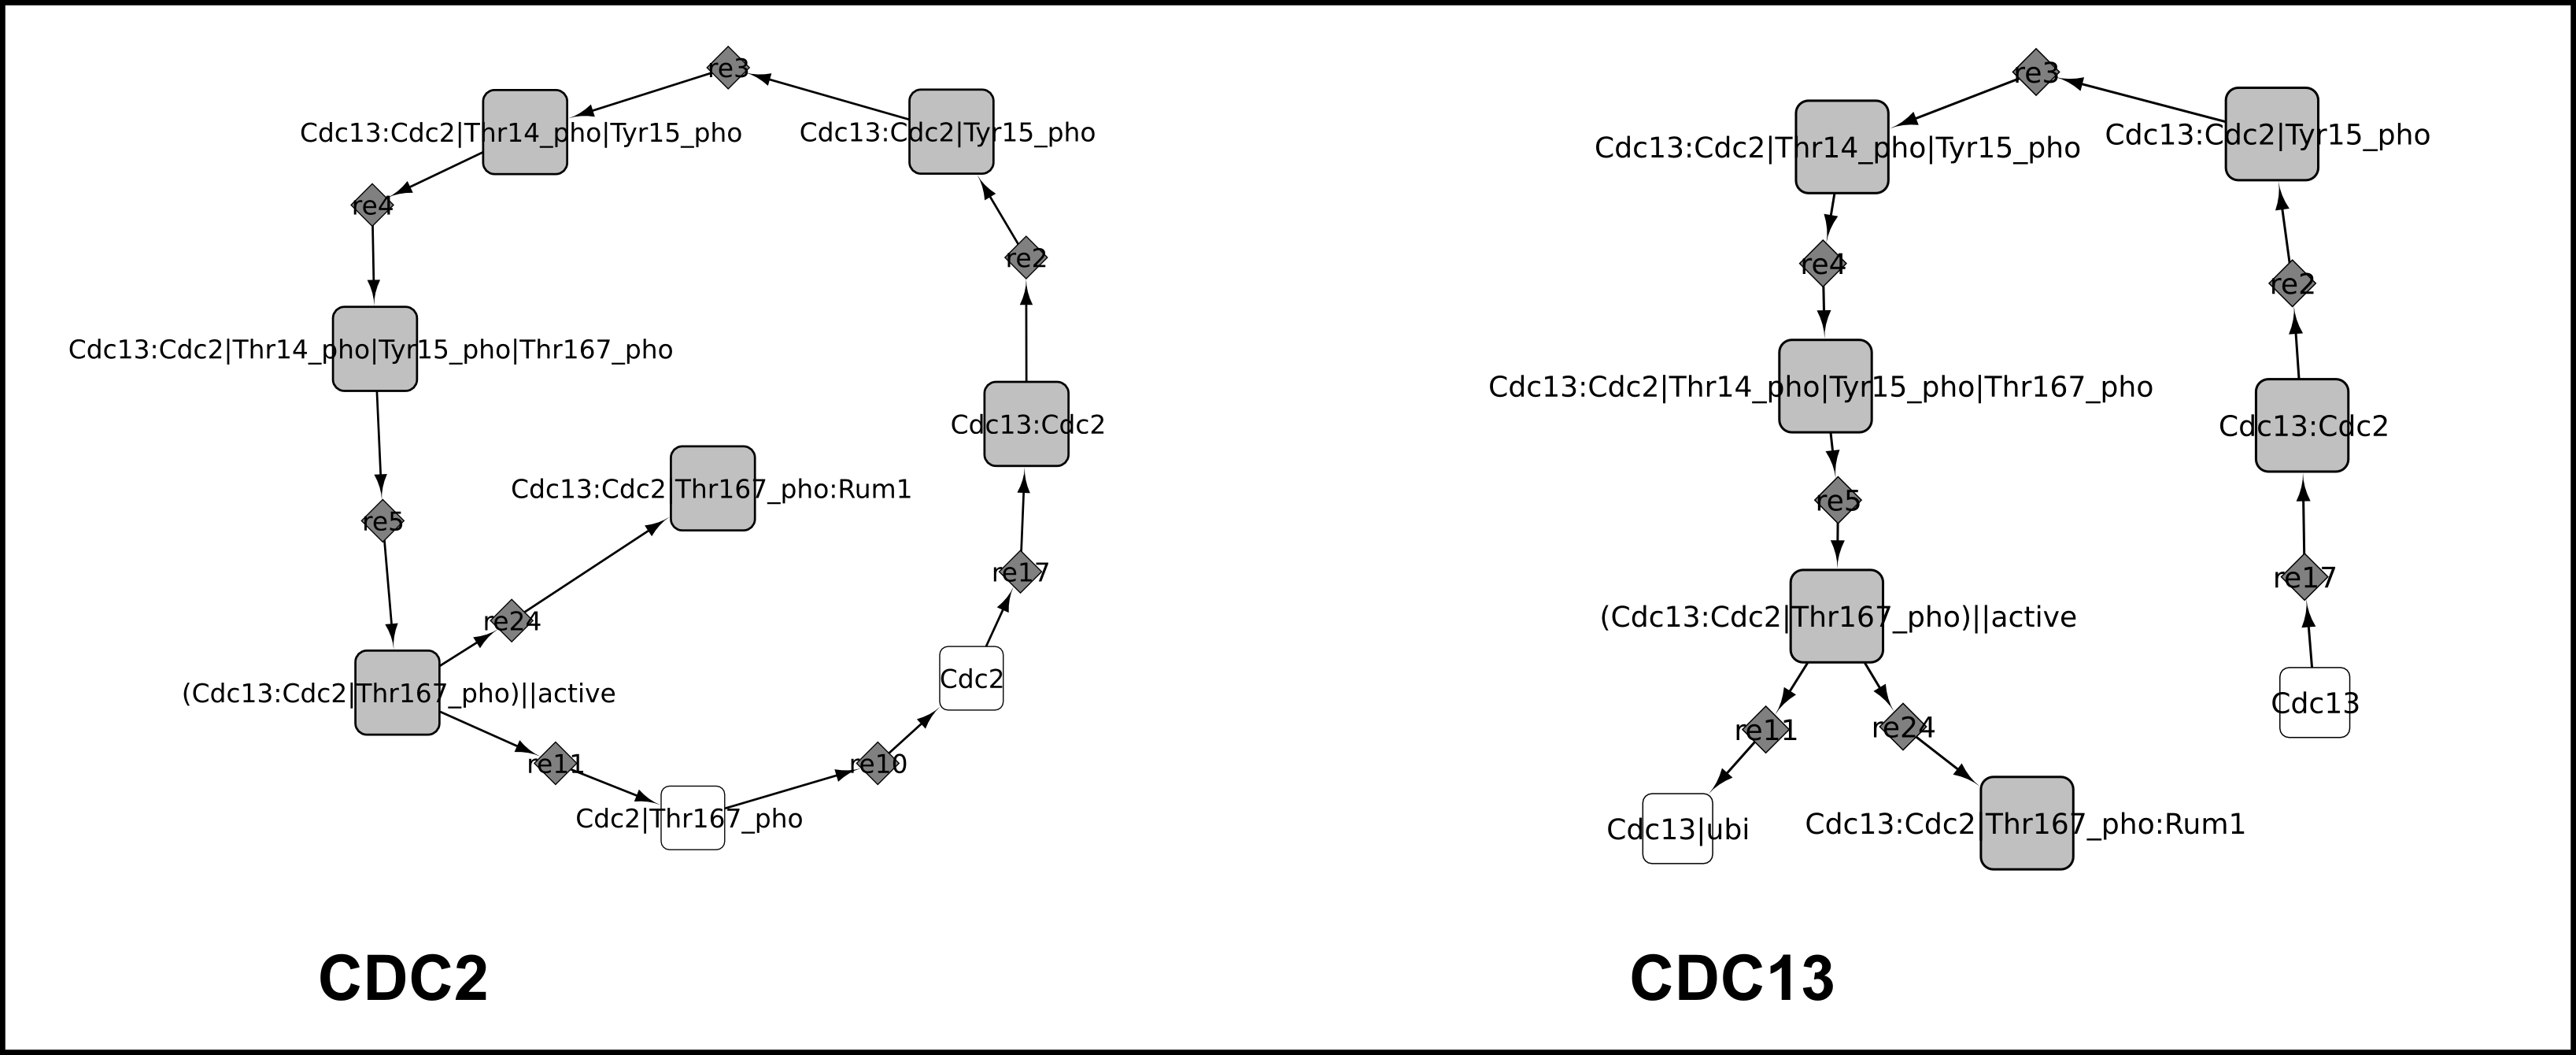
\includegraphics[width=0.7\textwidth]{figures/mat_cdc2_cdc13.png}}
\end{figure}


The cycle decomposition is splitting the network into relevant directed cycles
\cite{gleiss2001relevant}, using a modifed version of the algorithm of Vismara
and colleagues \cite{vismara1997union}. This procedure commonly shows the
different mechanisms in which the protein is playing a role. Care must
be taken when applying this approach, as the number of cycles can be huge for
large network structures. For example, it might be preferable to eliminate first
the network hubs, which are by definition highly connected, and also group short
cycles in larger subnetworks before applying the decomposition function.
Figure~\ref{mphasecdc25cycles} shows two
cycles involving CDC25 after a cycle decomposition.

\begin{figure}[h]
 \caption{\label{mphasecdc25cycles}  \textbf{CDC25 subnetworks.}
      Two cycles for the CDC25 protein found after the decomposition of the cell cycle network model of Novak et al. \cite{novak1998model}.}
 \center{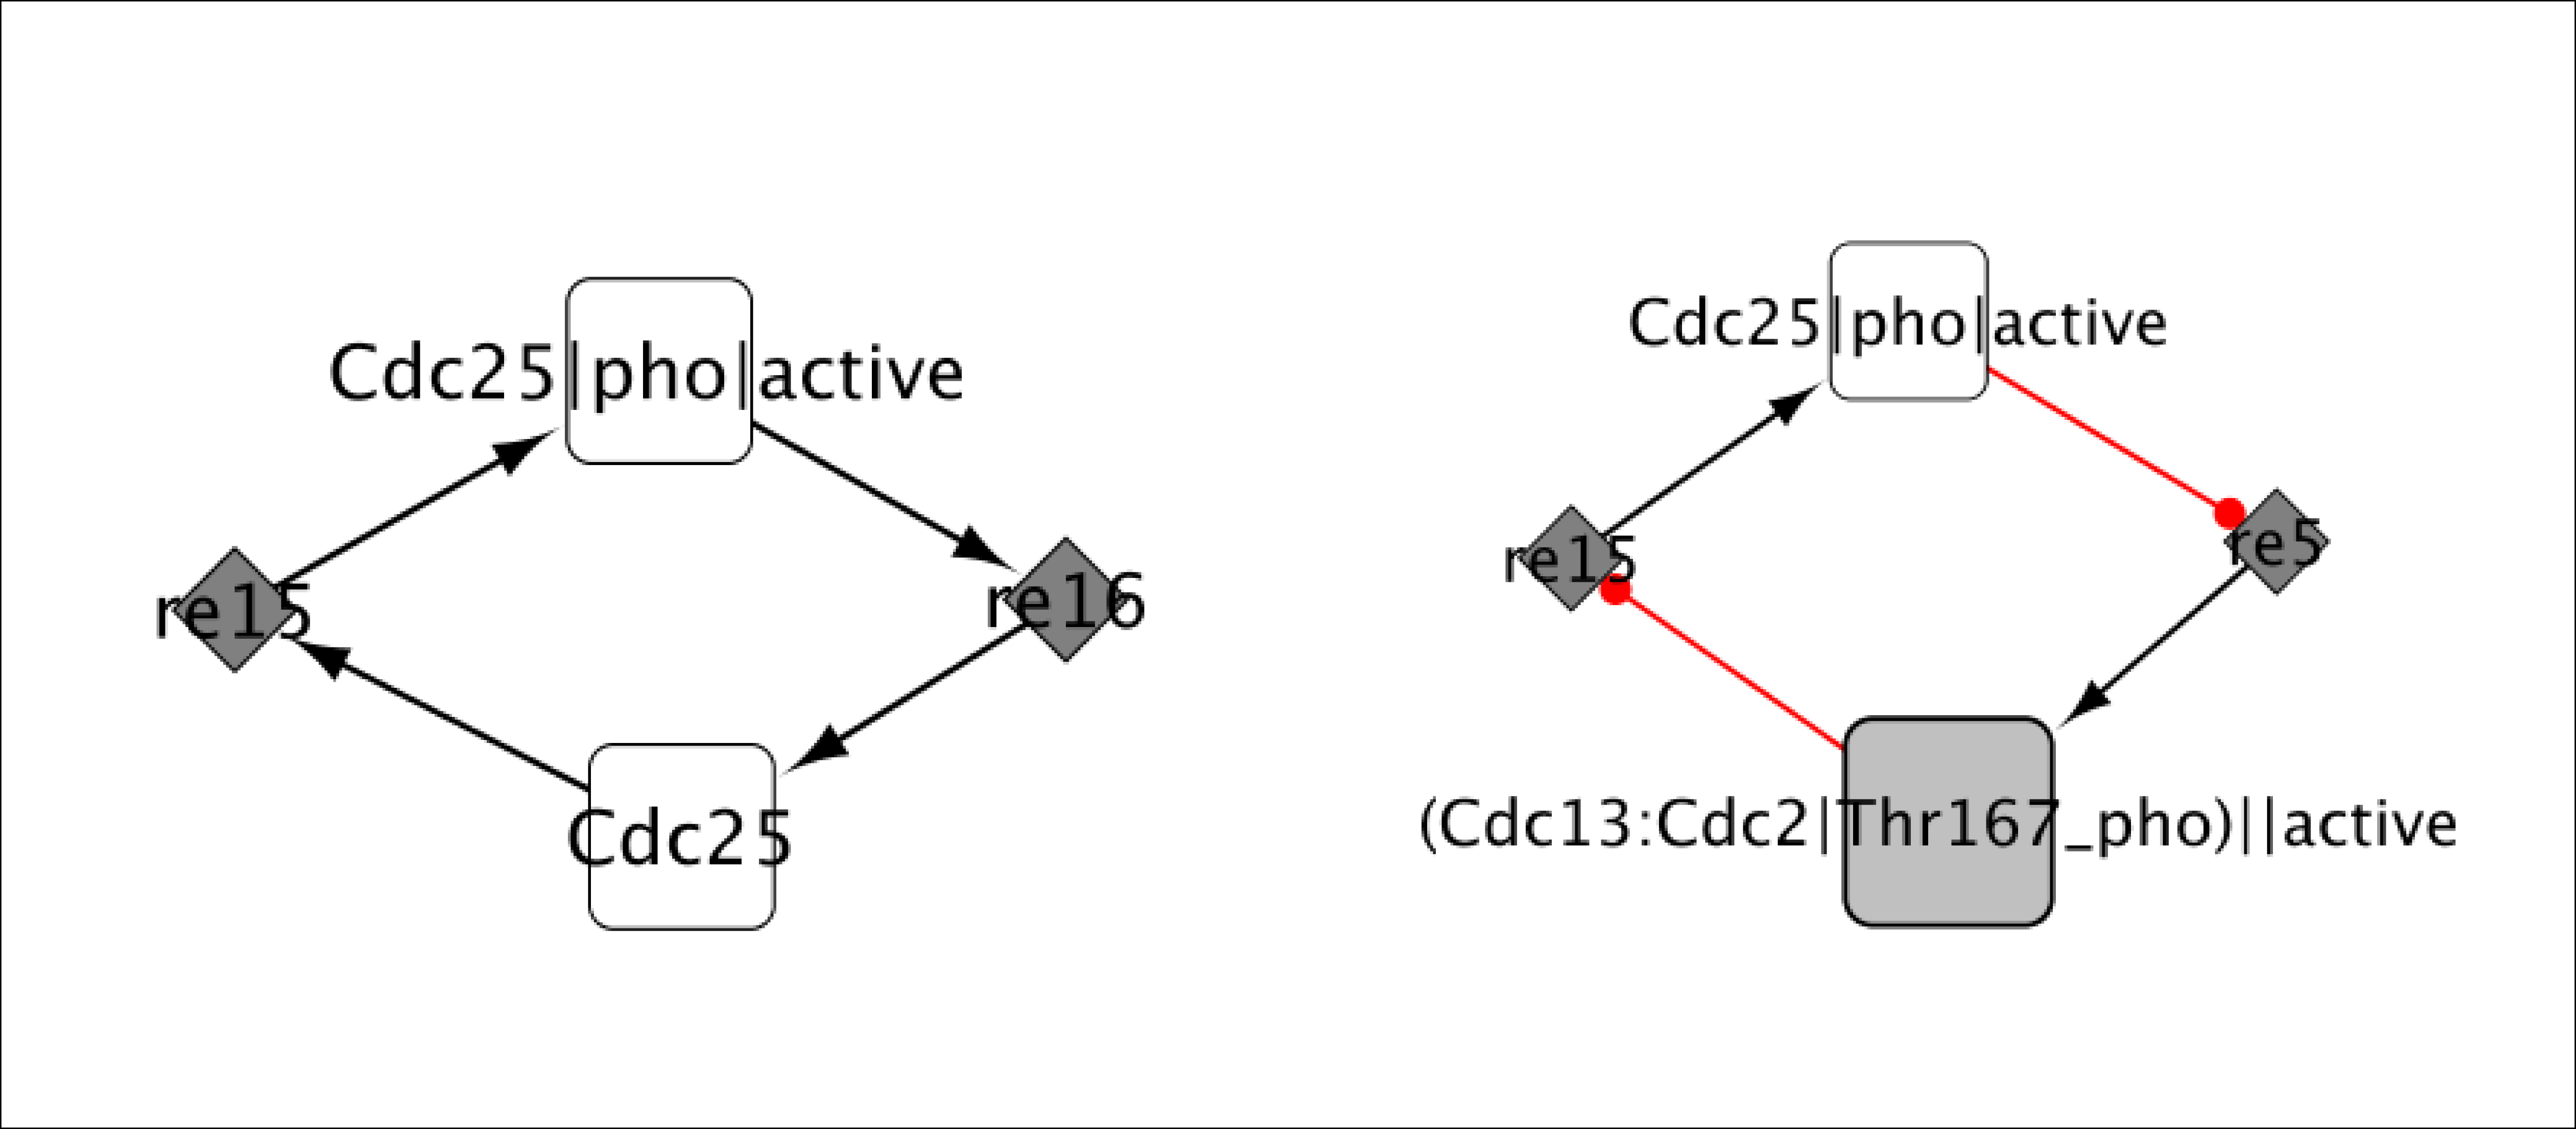
\includegraphics[width=0.7\textwidth]{figures/mphase_cdc25_cycles.png}}
\end{figure}

\subsubsection*{Path analysis algorithms}

BiNoM analysis functions also include several classical path analysis
algorithms, such as finding the shortest paths, the suboptimal shortest paths or
all non self-intersecting paths. The shortest path is calculated as the path having
the minimal sum of weights of the edges composing the path (Dijkstra's
algorithm) while the suboptimal path is constructed by removing all edges of
all shortest paths one by one, and finding the new shortest path. All non self-intersecting paths 
are those paths not containing loops (self-intersections). 
The user should be careful when using this procedure, as the number of paths between nodes can be
very large for big networks. In order to limit the number of paths found, BiNoM
allows to specify the maximal length of the path to be found.

Obviously, the result of some decomposition functions will result in subnetworks
that share some components, as it is for example often the case
with the decomposition in material components. Therefore, BiNoM also includes a
function to \emph{cluster} networks, based on common components such as protein
or protein complexes. To determine the size of the clusters, the user can
specify a percentage of intersection (ranging from 0 to 100\%) that will be used
as a threshold to create the clusters.

\subsubsection*{Pathway influence quantification algorithm}

In this version of BiNoM, we have introduced a novel approach to quantify the
effect of experimental data onto one or more target nodes for a given
network architecture, named the PIQuant score (Pathway Influence Quantification).
The target node can be a gene or a phenotype of interest, representing a more complex
biological function, such as cell proliferation or apoptosis.
For example, in the case of a network
with one source node and one target node,
the PIQuant score value will quantify the influence of the source node on the target
node, by taking into account experimental data values for the input nodes,
the path length and the sign of the path for a set of paths defined between the
source and the target node.
A positive or negative PIQuant score value is a quantitive theoretical
prediction of the over or underexpression of
the target node. For instance, let us consider that we have for a given network
experimental data corresponding to differential gene expression values (e.g.
disease/normal ratios).
In that case, a positive or a negative PIQuant score for a given phenotype
(output node) predicts quantitatively
that the phenotype would be respectively enhanced or inhibited. Furthermore, the
relative difference between two PIQuant score values also is also indicative of
a relative quantitative difference. Thus, the PIQuant score can be used to
compare the effects of two different experimental datasets on the same phenotype
(i.e using the same network), or to compare the effects of two different network
architectures on the same phenotype for one experimental dataset.


More formally, we can define a source node as \textit{annotated} when a signed real
number is assigned to the node, representing an experimental data value. For example, it
can be the expression ratio of a gene between a disease and a normal state,
obtained from transcriptomics profiling.
 A path $k \in \{1,\ldots , q\}$ is defined
as a the sequence of consecutive connected nodes
between a source node and a target node (without repetition of any node
or edge). We can extract a set of paths from source nodes to target nodes (indexed
from $1$ to $q$), by using various algorithms. In BiNoM, we propose three solutions to search for paths between the
source and target nodes (shortest paths, suboptimal shortest paths and all
non-intersecting paths, see previous paragraph). The activity
$\alpha_k$ of the path $k$ is defined as the annotation
of its source node. We define the sign $\sigma_k$
of the path $k$ as the product of the signs of every edge of the path and finally
the length $\lambda_k$ of the path $k$ as the number of edges in the path. We also
hypothesize that the longer the path is, the lesser the global influence will be
on the target node. This assumption has the advantage of being simple and does
not require extra parameters other than the influence network to be calculated.
The PIQuant score for a set of $q$ paths (from a set of source nodes, to a set
of target nodes) is defined as:

$$
 PIQuant_{Score} = \sum_{k=1}^{q} \alpha_{k} \sigma_{k} \frac{1}{\lambda_{k}}
$$

In the case of the network presented in Figure~\ref{piquantnetworks}a, let us
consider Ac the source node and Ph the target node and consider only the two
paths defined in the Figures~\ref{piquantnetworks}b and
~\ref{piquantnetworks}c. Given that the
node Ac is annotated by the value $2.0$, that the first path has a length
equal to 3, and that the second path has a length equal to 5, we can calculate the PIQuant score
of the node Ac to the node Ph as:

$$
 PIQuant_{Score} = 2 \cdot 1 \cdot \frac{1}{3} + 2 \cdot (-1) \cdot \frac{1}{5}
= 0.27
$$


Sometimes a path has one or more intermediate nodes that are annotated nodes
(i.e. for which we have experimental data values),
in addition to the source node.
In that case, the intermediate node is \textit{consistent} if the sign of its
annotation is the same as the sign of the source node annotation multiplied by
the sign of the
path from the source node to the intermediate node. If signs are opposite, the
node is \textit{inconsistent}.
A path is \textit{consistent} if each annotated intermediate nodes is
consistent. A path is \textit{inconsistent} if at least one intermediate node is
\textit{inconsistent}.
In other words, a path is inconsistent when the
sign of the experimental data value for a node is opposite to the sign
of the path.

For example, according to the network represented in Figure~\ref{piquantnetworks}c, there is an influence from Ac to Ph
that goes through D . But if this path
is functional, the annotation of node D should have the same sign as the annotation for node Ac, because
Ac activates D indirectly (i.e. the path from Ac to D has a positive sign). In this case, the sign of D annotation (the experimental value) is opposite to
the sign of Ac annotation, and therefore, the path from Ac to Ph that goes through D is inconsistent.

Practically, we offer the option to
keep or not the inconsistent paths for the calculation of the PIQuant score,
depending on how the user wants to analyze the calculations. An inconsistent
path could indicate that the path is not complete, or could also indicate that
the path is correct but not active under the precise conditions in which the
experimental data was generated, corresponding to a different context.

In the case mentionned above in Figure~\ref{piquantnetworks}c, if only consistent paths are kept, then the PIQuant score of Ac to Ph
becomes:

$$
 PIQuant_{Score} = 2 \cdot 1 \cdot \frac{1}{3} = 0.67
$$

This score is higher than the value previously obtained with all the paths, and can be interpreted in this case as a higher activation of the phenotype.

In more realistic situations, we would have multiple source nodes with different
 annotations, and also multiple target nodes representing phenotypes of
particular nodes of interest. We have implemented in BiNoM a set of functions
that allow users to select source nodes, select target nodes, and choose among
three different options for searching paths (shortest paths, optimal and
suboptimal shortest paths, all non-intersecting paths). The software is then
calculating PIQuant scores for every target node specified, taking into account
every possible path found by the algorithm. An interactive window is detailing
the PIQuant score results, both globally and for every path from the source
nodes to the output nodes. It is also possible to get a full text report
detailing all the calculations and the results. We describe a detailed
and concrete application of the PIQuant algorithm to a real biological network
in the Results section.

\begin{figure}[h]
 \caption{\label{piquantnetworks}  \textbf{A simple influence network.} The
network is composed of seven nodes and nine edges (a). The two paths (b,c)
extracted from this network start from the source node \textbf{Ac} and end at
the target node \textbf{Ph} (which denotes a phenotype of interest). The nodes
\textbf{Ac} and \textbf{D} are annotated using experimental data, and have the
values $2.0$ and $-1.0$ respectively.}
 \center{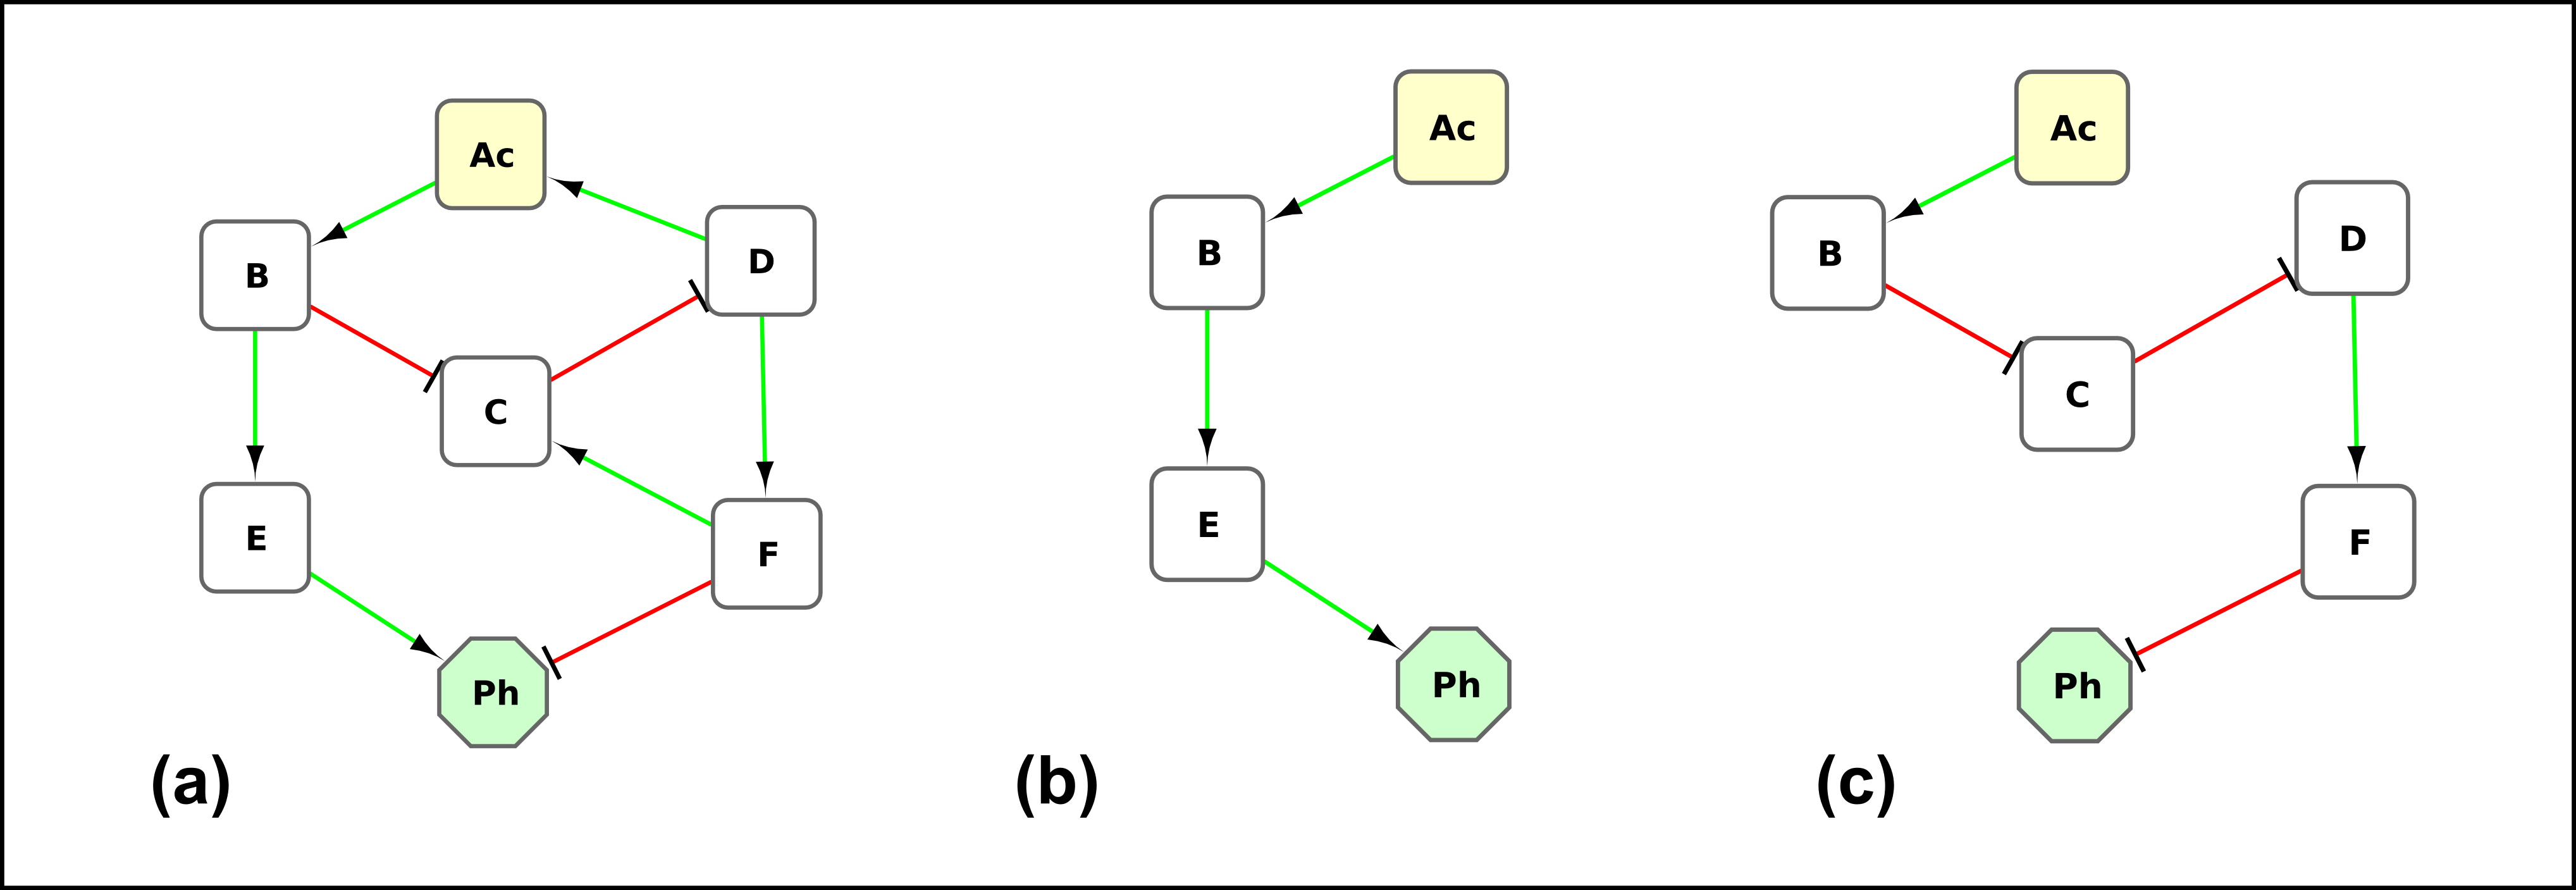
\includegraphics[width=0.7\textwidth]{figures/piquant_networks.png}}
\end{figure}

\subsection*{BiNoM BioPAX utils \& query}
The BioPAX format was primarily conceived as a standard facilitating the
exchange of data between various database systems \cite{demir2010biopax}. As a
consequence, this format was designed first to be machine-readable, but was not
intended
to be edited and modified by biologists. Furthermore, due to its adoption by
large biological knowledge repositories, some BioPAX files can be really big,
such as the \textit{Homo sapiens} network from the reactome database
\cite{joshi2005reactome} that has more than 6,000 reactions involving more than
8,000 chemical species (proteins, RNA molecules, metabolites, etc.).

BiNoM implements a set of functions precisely aiming at allowing end users to
easily visualize and modify BioPAX files. To the best of our knowledge, there is
no other software package allowing to view, query and edit BioPAX files than
BiNoM at the moment. The functions are using
Java class introspection techniques to build a BioPAX class tree. Then, the
content of the file can easily be accessed. For example, Figure~\ref{biopaxtrailprop} shows
all the information linked to the TRAIL protein, after a call to the
BioPAX property
editor function of the BiNoM menu has been made. Details are given in the BiNoM manual on how
to display valid attributes, edit them, and how to visualize the
complete BioPAX tree.


\begin{figure}[h]
 \caption{\label{biopaxtrailprop}  \textbf{Extra information linked to the TRAIL protein.}
      The information is automatically extracted from the BioPAX file upon
import with the BiNoM I/O functions.}
 \center{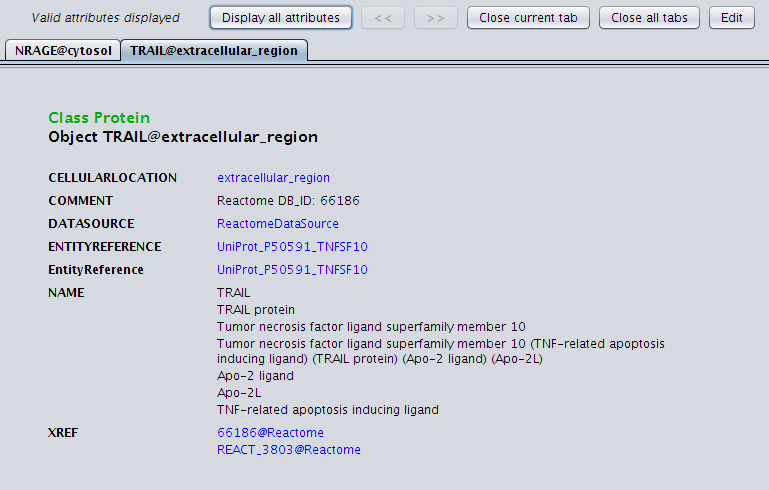
\includegraphics[width=0.7\textwidth]{figures/biopax_trail_prop.png}}
\end{figure}


The BioPAX Query functions in BiNoM allow the user to work with huge
BioPAX data files and extract the relevant information, by querying an index and
retrieving data from it. The index corresponds to a mapping of the content of
the BioPAX file on a labeled graph (an index file is created and saved, using
the XGMML format). Various statistics can be displayed on the content of the
index, such as the number of proteins, complexes, reactions, publications, etc.
To start extracting relevant information, the user can query the index by gene
name (and/or by any synonym of the gene) and start building a network centered
around this molecule of interest. The extension of the network is done by adding
different types of entities: complexes where the molecule of interest is
involved, chemical species, reactions (with the possibility of including all the
sources and targets of the reactions) and related publications. Figure~\ref{smaccomplexes}
illustrates an example of a small network extracted from the human apoptosis
pathway downloaded from the Reactome database \cite{joshi2005reactome}, and
centered on the SMAC protein, with all the protein complexes in which
this protein is involved and that were added using the BiNoM BioPAX Query functions.

\begin{figure}[h]
 \caption{\label{smaccomplexes}  \textbf{SMAC pathway subnetwork.}
      Subnetwork extracted from the human Apoptosis pathway, starting with the
SMAC protein (white square) and expanding to all protein complexes where this
molecule is involved (grey squares) using the BiNoM Query functions.}
 \center{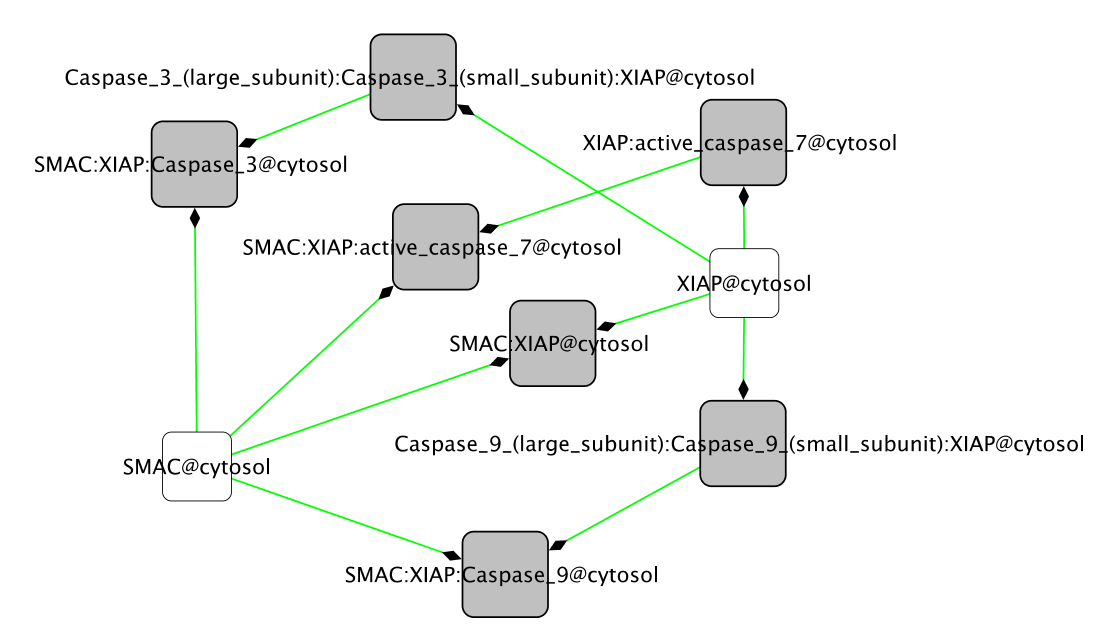
\includegraphics[width=0.7\textwidth]{figures/smac_complexes.png}}
\end{figure}

\subsection*{BiNoM Module manager}

To facilitate the visualization of large molecular networks, we propose a set of
functions that simplify them by creating modules from selected parts of the
large network. This task, that we call \emph{modularization}, is a
semi-automatic procedure, where biological expert knowledge is used to assure
the coherence of the newly created modules.

Most of the modules represent a detailed
sequence of events that occur with a particular protein or protein complex,
whose name can then be used to represent the whole module. This way, a
simplified representation of a complex map can be produced, using the modules
and their relationships as an abstracted version of the comprehensive network
\cite{calzone2008comprehensive}.

To facilitate the creation and management of modules, we have used in this
version of BiNoM a new feature introduced in recent versions of Cytoscape (as of
version 2.7) \cite{cline2007integration}, known as \emph{nested} networks. This
feature allows to embed any cytoscape network in a (meta)node. It was
introduced to allow the creation of network hierarchies and circular
relationships. In BiNoM, we use this feature to facilitate the process of
modularization of a large network. The BiNoM module manager integrates
functions that allow to easily create a network from a list of subnetworks,
packing individual nodes, merging different subnetworks, displaying information
about metanodes and calculating the intersection between subnetworks.

\subsection*{BiNoM Utilities}
This set of functions corresponds to various small utilities that are not
implemented in Cytoscape yet, but might be very useful for the analysis and
manipulation of networks. For example, it is possible to automatically select
the edges between two nodes, generate the network corresponding to the double
network differences between two networks A and B, or update all the subnetworks of
a session after some changes have been made to the initial one. The BiNoM Utilities also implement
clipboard functions, giving the possibility to copy, add and paste
selected nodes and edges and also to show the clipboard content.


\section*{Results and Discussion}
We propose to study a reaction network focusing on the transition from G1 phase
(growth phase) to S phase (DNA replication phase) of the cell cycle
\cite{calzone2008comprehensive} as an example of the use of BiNoM functions.

The network published in \cite{calzone2008comprehensive} describes in
biochemical details the regulation of the well-known and charaterized tumor
suppressor gene retinoblastoma (RB or RB1). The product of this gene operates at
the heart of the cell cycle, acting as a signal transducer, connecting the
cell cycle with the transcriptional machinery. The pathway in which RB is
acting is disrupted in many human tumor types \cite{weinberg1995retinoblastoma}.
The comprehensive map of the RB/E2F network was built using CellDesigner
\cite{funahashi2003celldesigner}. It lists 80 proteins, 208 chemical species, 165
interactions, 176 genes, and recapitulates more than 350 publications, including
information from different cellular types, thus making the map a generic map of
the cell cycle regulation. It is composed of two main compartments: the cell,
containing the cytoplasm, the nucleus and the nucleolus, in which the
biochemical interactions such as association, dissociation, (de)phosphorylation,
(de)acetylation, degradation, etc. take place; and the genes, which lists the
target genes of the main transcription factors of the map, the E2F family
members.
A thorough description of the model, the methods used to build it and create
simplified versions of it along with an interactive (clickable) map are
available on our website
(\url{http://bioinfo-out.curie.fr/projects/rbpathway/interactive/rb_network.html/}).

For the study presented here, we chose to concentrate on the G1 to S transition. We
used the intersection of the 208 chemical species
of RB/E2F network and the 280 chemical species listed in Reactome \cite{joshi2005reactome} for the G1-S transition
(referred to as \emph{Mitotic G1 G1/S phases} in Reactome). The resulting
subnetwork contains 38 proteins, 98 chemical species, and 100 biochemical
reactions (Figure~\ref{g1s}).

\begin{figure}[h]
 \caption{\label{g1s}  \textbf{G1/S network.}
	Overview of the G1 to S transition network, corresponding to the intersection of
RB/E2F network and G1/S network extracted from Reactome.}
 \center{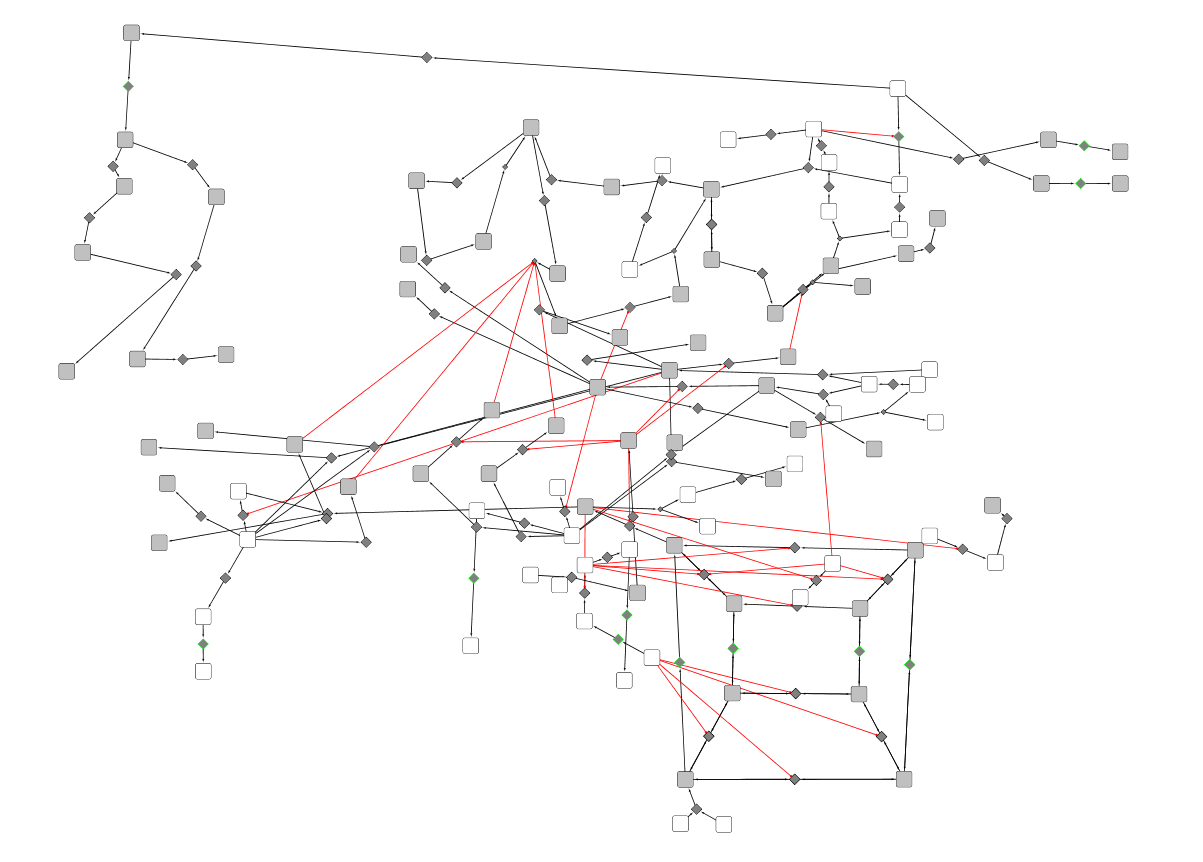
\includegraphics[width=0.85\textwidth]{figures/G1S.png}}
\end{figure}

This map contains a lot of valuable information but rather difficult to extract. We present two
ways to get some biological insight from this map, by using BiNoM functions. The first one consists of
transforming the reaction network into an influence network in order to analyze
experimental data on it. The second one implies a simplification of the comprehensive map by
applying a method of reduction of the numerous interactions into modules without
losing any content from the original map.

\subsection*{Application of PIQuant on an influence network.}
PIQuant algorithm can be used to perform a quantitative analysis on an influence
network. In order to translate the G1/S reaction network into an influence network, we used
a tool developed by the team of BIOCHAM \cite{calzone2006biocham} that is
available online (\url{http://contraintes.inria.fr/~soliman/cd2dot.html}). In order to translate a reaction network into an influence network, the first one is 
pre-processed accordingly to simple rules: (1) BIOCHAM deletes all linear
degradations and syntheses, (2) all intermediary chemical species with only one input and
one output are suppressed, (3) if the reactions of synthesis and degradation of
the chemical species deleted in (2) have distinct inputs and outputs, then these reactions
can be merged, and (4) if they have the same chemical species as input/output, then the reaction is a
reversible reaction and is replaced by a degradation. The further
translation is based on constructing Jacobian corresponding to the pre-processed reaction graph
and analyzing the signs of its entries \cite{fages2008frontiers}. Description and an example of such a conversion is
available in \cite{calzone2011calamar}.

We applied PIQuant to the resulting influence network of the G1/S transition of
the cell cycle (Figure~\ref{InflAnnotNet}). We selected three target nodes as
markers of the G1, S and M
phases of the cell cycle. For the experimental data, we used expression data
from a study of 57 bladder cancer
tissue samples compared to 4 normal samples \cite{stransky2006regional}. For
each gene, the differential expression between tumor and normal tissue
is assessed by a t-test. The t-test statistic value is used as the annotation
for each gene. We selected the 19 nodes for which we had experimental data
values as source nodes (complexes are selected if one of the members for which
we had a experimental value had no unbound state in the network).

Then, we constructed a text file listing nodes of the influence network
and their annotation and we imported this file using the Cytoscape function
``Import $>$ Nodes attributes''
in the Cytoscape session of the influence network.
Figure~\ref{InflAnnotNet} represents this influence network after its import.


\begin{figure}[h]
  \caption{\label{InflAnnotNet} \textbf{Annotated influence network.}
    Influence network of the cell cycle G1/S transition generated by BIOCHAM. Colors represent
differential
expression obtained from transcriptomic data compared to normal tissue. Color
intensities are proportional to the t-statistic values (red values indicate
positive values corresponding to an activation, green values indicate negative
values corresponding to an inhibition). The three grey nodes are markers for the
different cell cycle phases: G1 (pRB\_star), S (CDK2/Cyclin E1 complex phosphorylated), M (CDC2/Cyclin E1 complex phosphorylated).}
  \center{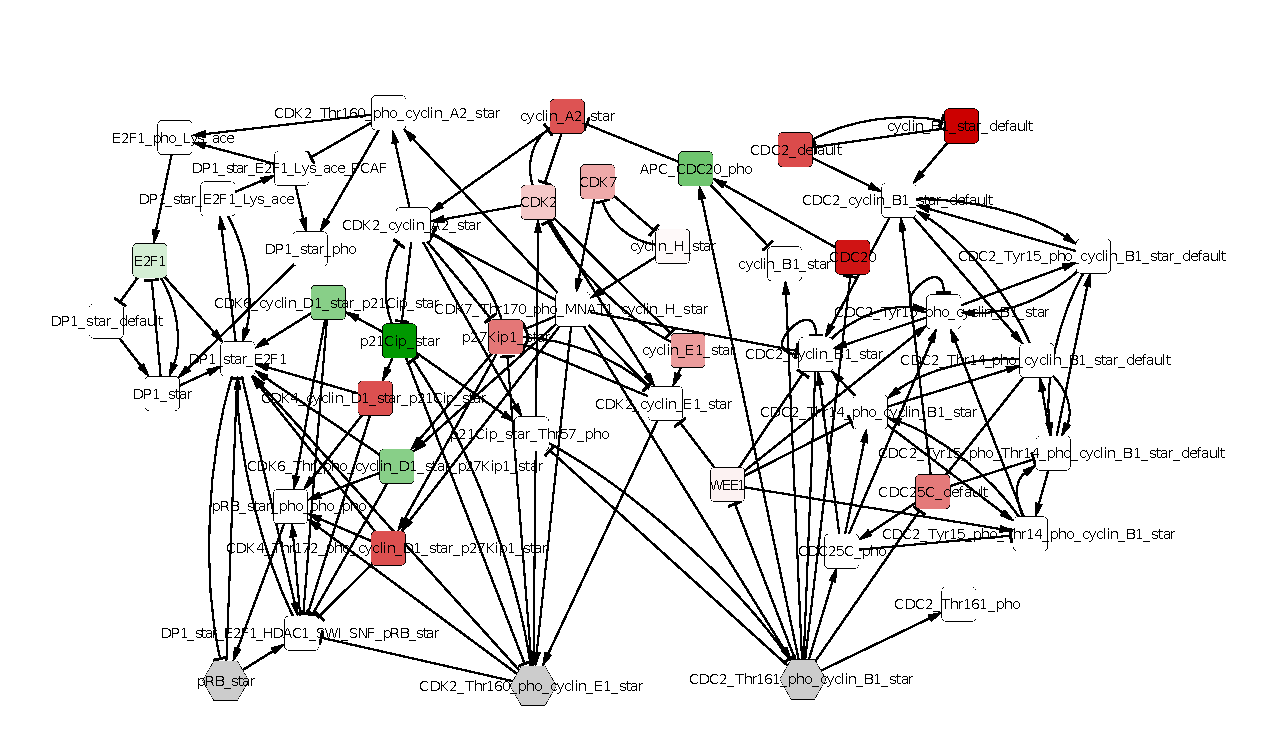
\includegraphics[width=0.85\textwidth]{figures/Cell_cycle_Expr.pdf}}
\end{figure}

PIQuant is applied to this network and its annotation, by using the function
``Plugins $>$ BiNoM 2.0 $>$ BiNoM Analysis $>$ Path Influence Quantification
analysis''. The PIQuant score is calculated for each association
between a source node and a target node (the list of nodes and all the PIQuant
score values are available as supplementary table 1). We selected the option ``optimal and
suboptimal shortest path'' as the algorithm to extract the paths. We ran a
significance test and got the report table. In this report, the ``Node influence
table'' represents the global PIQuant score from each annotated source node to
each cell-cycle phase marker. Those values are
represented as a heat map in Figure~\ref{PIQuantHeatMap}. We can see that most
genes, in cancer cells compared to normal cells, influence positively the M and S phases (red
coloring on the heatmap), indicating an enhanced proliferation for tumor cells.
Compared to Figure~\ref{InflAnnotNet}, where the coloring represents only the
experimental data values, we can see that the PIQuant score is integrating the
influence of the network architecture and the experimental data, thereby
providing a better and more accurate picture of the biological response.


\begin{figure}[h]
  \caption{\label{PIQuantHeatMap} \textbf{Heat map representation of the PIQuant
scores.}
    The map shows the results of the PIQuant algorithm applied to the G1/S
influence network. Color intensities are proportional to PIQuant score (red color indicates a positive
value; i.e an activation, the green color indicates a negative value, i.e. an
inhibition).
Each line represents a source node while each column represents a cell-cycle
phase.}

\center{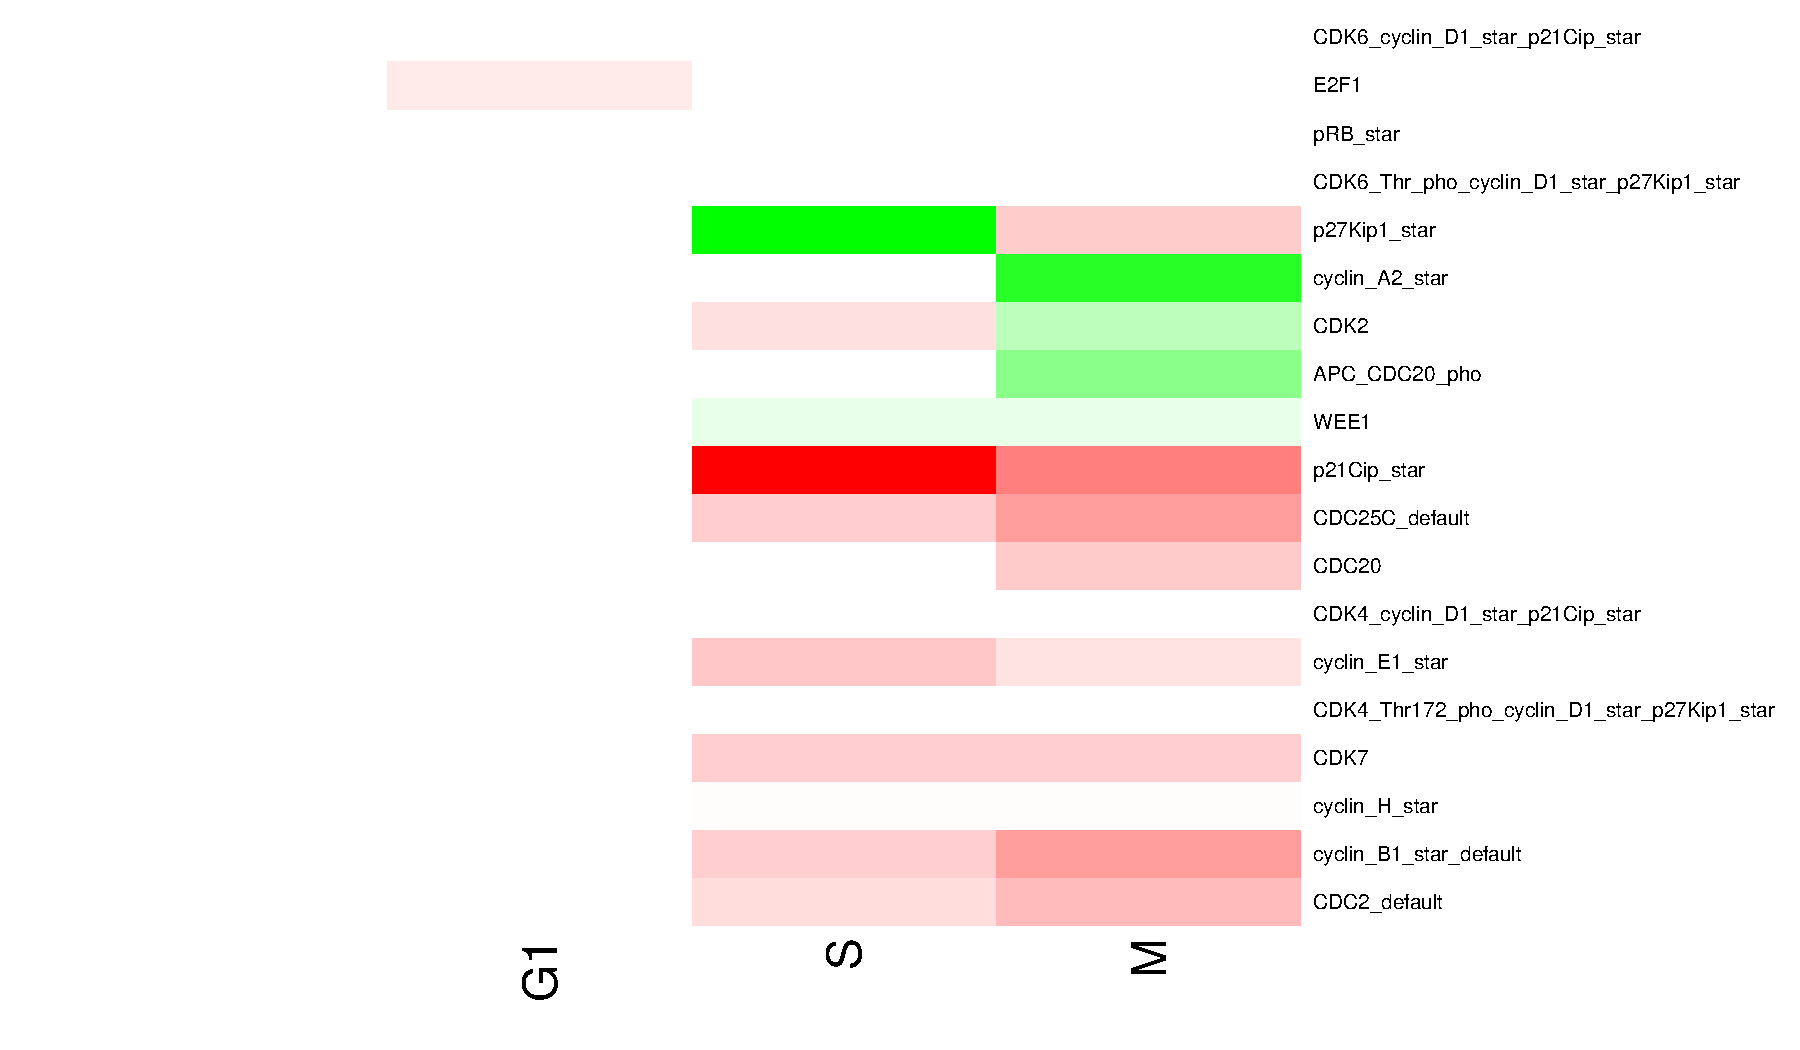
\includegraphics[width=0.8\textwidth]{figures/heatmapPathInfluence.pdf}}
\end{figure}



\subsection*{Modularization}

The raw G1/S network is very detailed and may be hard to read at a first glance.
To facilitate the analysis of the content, we propose to organize the reaction
network as a modular network. The chemical species are clustered in groups, referred to
as modules, in an semi-automatic manner, using BiNoM functions and biological
knowledge. Each module represents in fact a
sequence of events occuring with a particular protein. The modules are then
linked by activating or inhibiting influences according to the information
contained in the original diagram or derived from previous biological knowledge.

Briefly, we first decomposed the global network into its different components,
by using name semantics to isolate the subnetworks in which
each protein is involved. The 36 networks that are created this way may share a
lot of common chemical species, so we went further
by clustering the subnetworks having at least 25\% of common chemical species. We renamed
the 7 clusters obtained with a name that illustrates the content and the main
function of the clusters (such as E2F1\_RB, Wee1, etc.). Then, we checked the
content of each module, making modifications if necessary by adding or deleting nodes.
For example, the module E2F1\_RB is
further decomposed in three different modules containing the proteins RB, E2F1
and E2F6. Finally, we generated a modular view of all the individual modules.
BiNoM links the modules if they share components or edges. These edges are then
interpreted as activation or inhibition by the user (not shown here). Our final
modular view is composed of 9 modules, with 22
edges connecting them (Figure~\ref{g1smodular}). A detailed tutorial on the
construction of this modular network using BiNoM is described in the
supplementary methods.


\begin{figure}[h]
 \caption{\label{g1smodular}  \textbf{Modular view of the G1/S network.}
	Modular representation of the G1/S network, created by using a set of
different BiNoM functions. Each node (pictured as a green octagon), represents a
different module, or subnetwork. The edges connecting the modules represent the
 known influences between modules. }
 \center{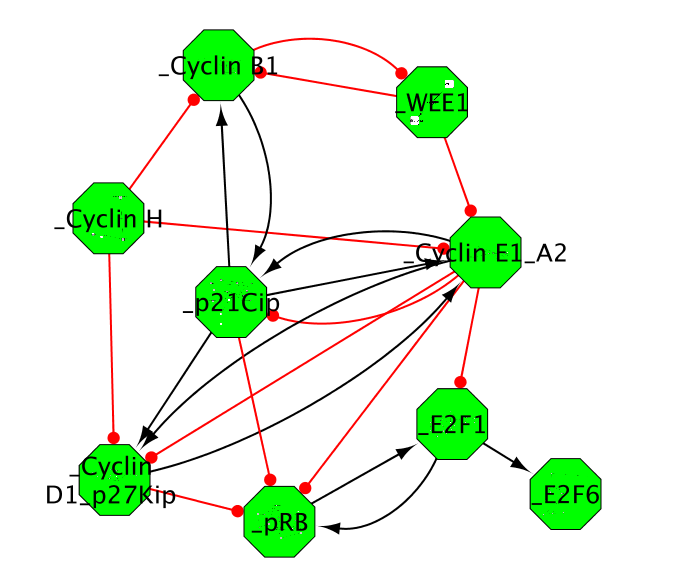
\includegraphics[width=0.7\textwidth]{figures/G1S_modular.png}}
\end{figure}

The modular view offers a simplified visualization of the complex network. The
obtained model is more abstract but highlights some aspects that may not be
evident from the comprehensive reaction network. For instance, it brings into relief some
feedbacks, positive, negative or feedforward, involving the major players of the
cell cycle, and prepares the network for mathematical modeling. The translation
of this modular network into a Boolean model is indeed straightforward.

\section*{Conclusions}

Building a suitable model for systems and mathematical biology is a multi-step
process, beginning with the collection of biological knowledge and progressing
towards the formalization of a network and its translation in mathematical
terms. BiNoM was designed to help during the intermediate steps of this process,
by providing a convenient access to some standard Systems Biology
representations such as BioPAX, by giving the possibility to manipulate the
network by applying various algorithms (mostly based on graph theory)
and map biological data to it. BiNoM is clearly not a tool for numerical
simulations, but it provides functions to export final networks to the SBML and
GINsim file formats (through the GINsim Cytoscape plugin for Boolean modeling), facilitating the
import into various numerical simulators.

The current development of BiNoM includes new functions such as merging several
independent networks into one, finding minimal intervention sets to disrupt or modify the
signaling flow from a set of source nodes to a set of target nodes (OCSANA algorithm, \cite{Vera-Licona2012OCSANA}), ability to
generate a code for web-based representations of biological networks using the
Google Map API, with a possibility to discuss and curate the network through a dedicated web-blog 
(NaviCell software, http://navicell.curie.fr)


\section*{Availability and requirements}

\begin{itemize}
\item Project name: BiNoM
\item Project home page: \url{http://binom.curie.fr/}
\item Operating system(s): Platform independent
\item Programming language: java
\item Other requirements: java 1.5 or higher, Cytoscape 2.7 or higher
\item License: GNU LGPL
\item Any restriction to use by non-academics: none
\end{itemize}




% \section*{Section title}
% \subsection*{Sub-heading for section}
% \subsubsection*{Sub-sub heading for section}
% \subsubsection*{Sub-sub-sub heading for section}

\bigskip

%%%%%%%%%%%%%%%%%%%%%%%%%%%%%%%%
%\section*{Author's contributions}
%    Text for this section \ldots



%%%%%%%%%%%%%%%%%%%%%%%%%%%
\section*{Acknowledgements}
  \ifthenelse{\boolean{publ}}{\small}{}
  EB, LC, DR, GS, EmB and AZ are members of the team ‘‘Computational Systems Biology of
Cancer,’’ Equipe labellisée par la Ligue Nationale Contre le Cancer.

%%%%%%%%%%%%%%%%%%%%%%%%%%%%%%%%%%%%%%%%%%%%%%%%%%%%%%%%%%%%%
%%                  The Bibliography                       %%
%%                                                         %%
%%  Bmc_article.bst  will be used to                       %%
%%  create a .BBL file for submission, which includes      %%
%%  XML structured for BMC.                                %%
%%  After submission of the .TEX file,                     %%
%%  you will be prompted to submit your .BBL file.         %%
%%                                                         %%
%%                                                         %%
%%  Note that the displayed Bibliography will not          %%
%%  necessarily be rendered by Latex exactly as specified  %%
%%  in the online Instructions for Authors.                %%
%%                                                         %%
%%%%%%%%%%%%%%%%%%%%%%%%%%%%%%%%%%%%%%%%%%%%%%%%%%%%%%%%%%%%%

\newpage
{\ifthenelse{\boolean{publ}}{\footnotesize}{\small}
 \bibliographystyle{bmc_article}  % Style BST file
  \bibliography{binom2} }     % Bibliography file (usually '*.bib' )

%%%%%%%%%%%

\ifthenelse{\boolean{publ}}{\end{multicols}}{}

%%%%%%%%%%%%%%%%%%%%%%%%%%%%%%%%%%%
%%                               %%
%% Figures                       %%
%%                               %%
%% NB: this is for captions and  %%
%% Titles. All graphics must be  %%
%% submitted separately and NOT  %%
%% included in the Tex document  %%
%%                               %%
%%%%%%%%%%%%%%%%%%%%%%%%%%%%%%%%%%%

%%
%% Do not use \listoffigures as most will included as separate files

%\section*{Figures}
%  \subsection*{Figure x - title}
%      Description.


%%%%%%%%%%%%%%%%%%%%%%%%%%%%%%%%%%%
%%                               %%
%% Tables                        %%
%%                               %%
%%%%%%%%%%%%%%%%%%%%%%%%%%%%%%%%%%%

%% Use of \listoftables is discouraged.
%%
%\section*{Tables}
%  \subsection*{Table 1 - Sample table title}
%    Here is an example of a \emph{small} table in \LaTeX\ using
%    \verb|\tabular{...}|. This is where the description of the table
%    should go. \par \mbox{}
%    \par
%    \mbox{
%      \begin{tabular}{|c|c|c|}
%        \hline \multicolumn{3}{|c|}{My Table}\\ \hline
%        A1 & B2  & C3 \\ \hline
%        A2 & ... & .. \\ \hline
%        A3 & ..  & .  \\ \hline
%      \end{tabular}
%      }



%%%%%%%%%%%%%%%%%%%%%%%%%%%%%%%%%%%
%%                               %%
%% Additional Files              %%
%%                               %%
%%%%%%%%%%%%%%%%%%%%%%%%%%%%%%%%%%%

\section*{Additional Files}
  \subsection*{Supplementary methods}
	Detailed tutorial for the creation of a modular view of the G1/S network using BiNoM functions.
  \subsection*{Supplementary table 1}
	PIQuant score values for all the source nodes (rows) and all the target nodes (columns) of the G1/S influence network.

\end{bmcformat}
\end{document}







